\section{Results}
\label{test}
DRD and TTS has informed me that the DOGS system has not previously been tested in a simulation environment. The initial project proposal by Steen Lauritzen of DRD was to perform such a test in the Vissim simulation tool, described in sections \ref{vissim} and \ref{modelling}.

As part of this tests were performed to discover the effect of bus priority and to discover whether the uncontrolled green time displacements, which DOGS introduce during level change (see section \ref{dogs_offset}), can be remedied by choosing cycle-time specific offsets at level changes.

Only the morning period (7.00-9.00) was tested due time constraints and that, the fact that few differences in results were expected considering the similarities between morning and afternoon (15.00-17.00) we saw in section \ref{data}.
 
The overall conclusion is that the combined performance of the network is reduced when DOGS is running. This means that the positive effect for traffic traversing the arterial does not outweigh the penalties for crossing traffic. 
This is acceptable since DOGS, for political reasons, was sanctioned to perform a capacity redistribution from minor road (traffic from east- and west) to arterial traffic. However, tests show that this redistribution does not succeed in a convicing way and even increases queue lengths and delays for arterial traffic in some cases.

In section \ref{dogs_offset} I discussed how DOGS inadvertently alters the coordination as it increases the cycle time without compensating by implementing new offsets. The tests involving \textit{Modified DOGS} show that DOGS can be improved by choosing new offsets when the cycle time is changed.

For bus priority, although it is only enabled for a few of the involved intersections - and that the implemented priority logic could be more aggressive - there is a noticable effect.

The rest of this section explains the test setup and test scenarios I used to arrive at these conclusions. 

\subsection{Test Scenarios \& Setup}

Below are the six scenarios, which were tested:

\begin{enumerate}
\item Basic program
\item Basic program with bus priority
\item DOGS
\item DOGS with bus priority
\item Modified DOGS
\item Modified DOGS with bus priority
\end{enumerate}

In scenarios 1 and 2 DOGS is disabled effectively ignoring all detections (except for buses in scenario 2) and thus the signals will remain in the basic, morning program (see appendix \ref{app:signalplans}). These scenarios represent the situation before DOGS was introduced and as such constitute a comparison baseline.

In scenarios 3 and 4 DOGS is enabled and the capacity in the main direction is adjusted according to detector values as described in section \ref{dogs}. For Herlev both scenarios are "authentic" ie. they are being used today whereas for Glostrup only scenario 4 is authentic, since this area implements bus prioritization for 3 of 4 intersections.

Finally scenarios 5 and 6 are DOGS with per-level offsets. These scenarios are included to show what happens when DOGS use incorrect offsets and to emphasize that DOGS but can be improved by using per-level offsets. 
The optimization routine described in section \ref{optimization} is used to precalculate cycle-time specific offsets for each DOGS-controller signal controller. 
Apart from the varying offsets, the only other difference between \textit{modified DOGS} and \textit{original DOGS} is that level changes cannot occur after at least 3 cycles to allow the new offsets to come into effect. Original DOGS allows level change immediately after the previous level change is implemented and although, as the cycle time increase the longer the time between possible level changes, levels may still change quite frequently, preventing any offsets from coming into effect.

As DOGS will naturally cause decreased performance for the minor roads it was decided to split the dataset so that \textit{arterial} and \textit{minor road} traffic can be distinguished. 

\begin{description}
\item[Arterial] traffic is defined as traffic which enters an intersection from north or south and makes a throughgoing motion rather than turning off the arterial. 
\item[Minor road] traffic consist of all traffic from east and west making left- and right turns as well as crossing over the artery.
\end{description}

The results of the tests are measured by extracting average queue lengths and average delays for each intersection. These values are extracted using Vissim node evaluations, which are inserted for each of the twelve intersections.

All simulations were fitted to the traffic observed in the morning period from 7.00 to 9.00 and run 10 times with different seeds. All graphs shown in this section are based on average values over the 10 runs.

\subsection{DOGS}
The first set of results compares DOGS to the basic program and DOGS with modifications.

\subsubsection*{Average queue lengths}
Average queue length indicates, in units of length (m), the number of vehicles waiting to traverse an intersection ie. perform some turning motion, or go straight through, in the beginning of the green interval. 

When queues become too long \textit{spillback} occurs causing queues upstream. In the extreme event queues stretch back to the last upstream intersection blocking all entry into the intersection and effectively causes a gridlock.
Another spillback situation, although less severe - but more common, is when vehicles waiting for a left-turn fill up a dedicated left-turning lane and spill back into the main direction.

These situations are, of course, not desirable and thus the queue length is an important factor to observe.

The way DOGS work we can make some speculations on how queues will form. The intention of DOGS is to improve capacity for the arterial traffic while sacrificing some performance for the minor roads. So we expect queues to shorter for the main direction and longer for the side roads. This is a slightly risky strategy since the minor roads will usually have a short distance to the upstream intersection.

\begin{figure}[ht]

    \begin{minipage}[b]{0.5\linewidth}

\centering
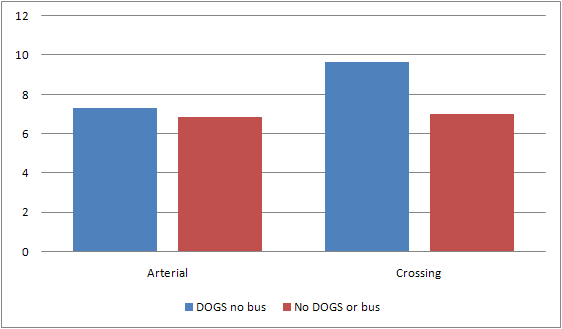
\includegraphics[scale=0.40]{aveq.png}
\caption{Average queue lengths for arterial and crossing traffic}
\label{fig:aveq}

    \end{minipage}
    \hspace{0.5cm}
    \begin{minipage}[b]{0.5\linewidth}

\centering
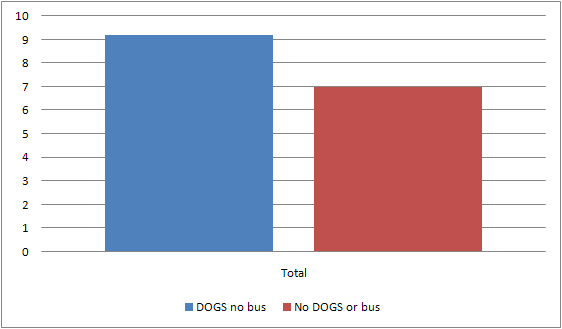
\includegraphics[scale=0.40]{aveq_total.png}
\caption{Average queue lengths for all traffic types (total performance)}
\label{fig:aveq_tot}

    \end{minipage}

\end{figure}

In Figures \ref{fig:aveq} and \ref{fig:aveq_tot} we see the average queue lengths for all intersections with and without DOGS, in both cases with no bus priority (since bus priority may cause increased queues and we want to save this aspect for later). The values behind these graphs are the averages for all intersections.

In Figure \ref{fig:aveq_detail} we see the total performance of each signal timing strategy per area. 

\begin{figure}[ht]
\centering
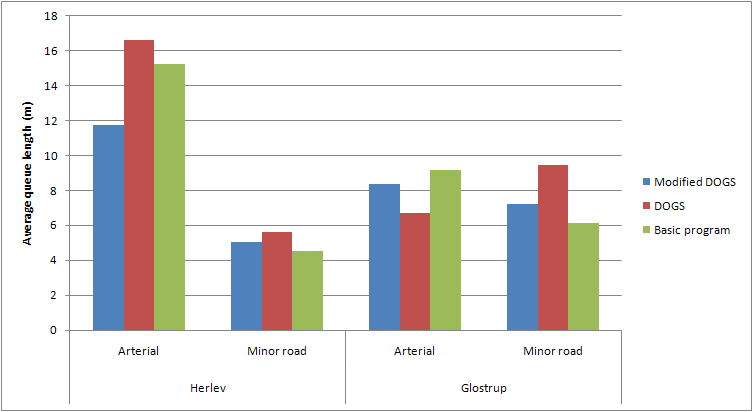
\includegraphics[scale=0.40]{aveq_total_area_vs_traffic-type.png}
\caption{Average queue lengths per area and traffic type}
\label{fig:aveq_detail}
\end{figure}

In Glostrup both DOGS variants outperform the basic program for arterial traffic. Original DOGS delivers about 20\% shorter queues on the artery than modified DOGS, which, in turn is about 10\% better than the basic program. For the minor roads, again both DOGS variants increase the queue lengths for minor roads but modified DOGS has an edge over DOGS in this case.

In Herlev DOGS actually increase the queue lengths for arterial traffic, compared to the baseline program, unlike modified DOGS, which bring a 25\% advantage over the baseline. For the minor road traffic we again see that, on average, this type of traffic experience longer queues however the difference is not as extreme as in Glostrup.

\begin{figure}[ht]
\centering
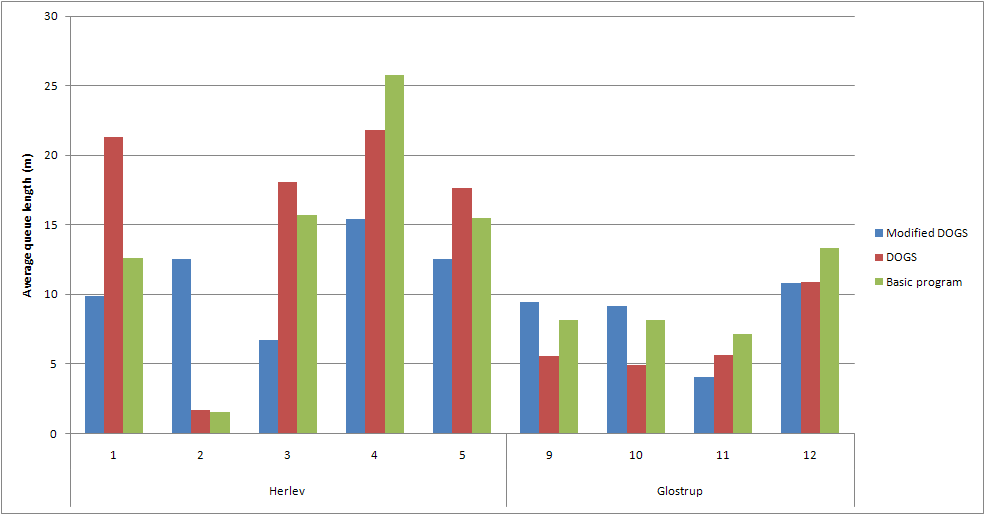
\includegraphics[scale=0.30]{aveq_intersection_arterial.png}
\caption{Average queue lengths per intersection for arterial traffic}
\label{fig:aveq_int_art}
\end{figure}

\begin{figure}[ht]
\centering
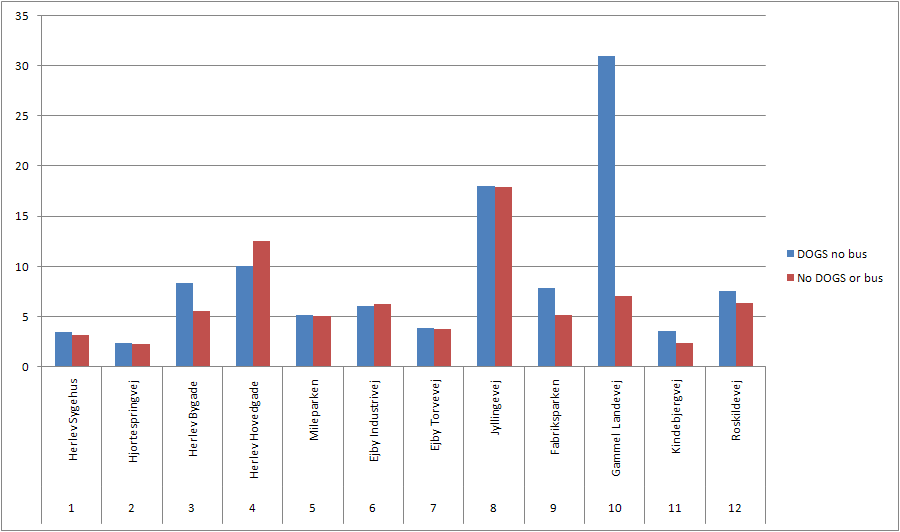
\includegraphics[scale=0.30]{aveq_intersection_crossing.png}
\caption{Average queue lengths per intersection for minor road traffic}
\label{fig:aveq_int_cross}
\end{figure}

(Since intersections 6 to 9 are not controlled by DOGS the performance is almost identical wether DOGS is enabled or not and are not shown for this reason.)

Figures \ref{fig:aveq_int_art} and \ref{fig:aveq_int_cross} shows the average lengths of queues forming at arterial and  minor road intersection approaches. We see that in the Herlev area only arterial traffic at Herlev Hovedgade gains an advantage under DOGS. On the other hand the Herlev Sygehus intersection performs almost twice as bad as it did without DOGS.

Modified DOGS outperforms DOGS and the basic program in all cases but Hjortespringvej, which deviates drastically from both DOGS and the basic program. In this case the optimization routine has chosen offsets, which yield good average performance for the area, sacrificing Hjortespringvej.

DOGS performs better in all Glostrup intersections yielding from 10\% at Kindebjergvej to almost 40\% reduced queue length at Gammel Landevej compared to the basic program. Here modified DOGS is outperformed by DOGS at Fabriksparken and Gammel Landevej by a margin og almost 50\%, and performs slightly worse than the basic program. At Roskildevej DOGS and its modified sibling is at par, both outperforming the basic program. Modified DOGS excels, however, at Kindebjergvej.

Looking at the performance for minor road traffic, the promised "sacrifices" are clearly visible. In Herlev there are slight increases of average queue length for intersections Herlev Sygehus, Hjortespringvej and Mileparken. Herlev Bygade suffer about 30\% longer queues under DOGS control - but 20\% less under modified DOGS control.

In Glostrup we see moderate performance variations for Fabriksparken and Kindebjergvej. Roskildevej and Gammel Landevej are more affected, Roskildevej suffering more than 40\% longer queues on average. In both cases modified DOGS is somewhat closer to the basic program, although still increasing queue lengths.

\subsubsection*{Average delays}
We conclude the comparison of DOGS and modified DOGS to the basic program by looking at the average delays experienced in each area for each traffic type. 

These are found in Figures \ref{fig:delay_arterial_herlev}-\ref{fig:delay_minor-road_glostrup} where we see the combined performance for intersections in the respective area versus time in seconds.

\begin{figure}[ht]

    \begin{minipage}[b]{0.5\linewidth}

\centering
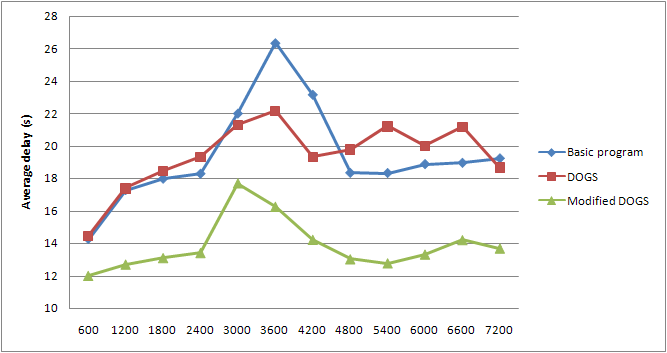
\includegraphics[scale=0.25]{delay_arterial_herlev.png}
\caption{Average delay for arterial traffic in Herlev}
\label{fig:delay_arterial_herlev}

    \end{minipage}
    \hspace{0.5cm}
    \begin{minipage}[b]{0.5\linewidth}

\centering
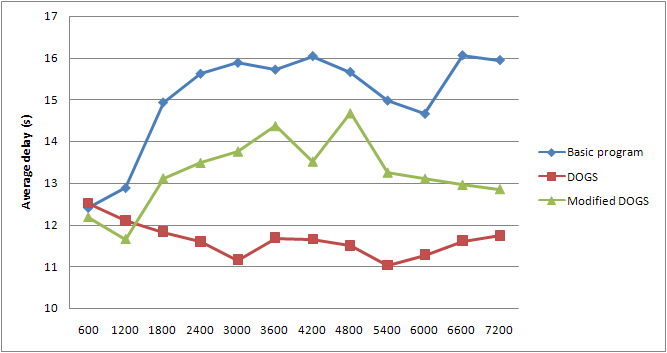
\includegraphics[scale=0.25]{delay_arterial_glostrup.PNG}
\caption{Average delay for arterial traffic in Glostrup}
\label{fig:delay_arterial_glostrup}

    \end{minipage}
    
        \begin{minipage}[b]{0.5\linewidth}

\centering
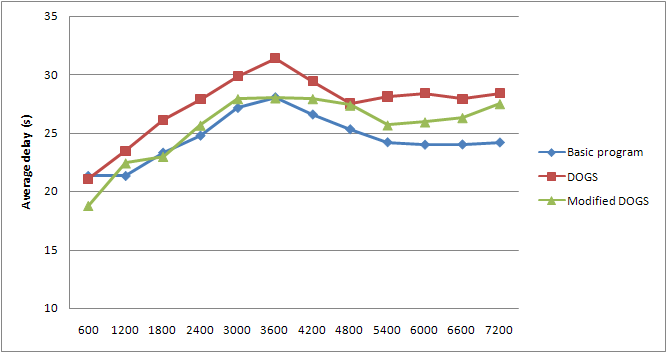
\includegraphics[scale=0.25]{delay_minor-road_herlev.PNG}
\caption{Average delay for minor-road traffic in Herlev}
\label{fig:delay_minor-road_herlev}

    \end{minipage}
    \hspace{0.5cm}
    \begin{minipage}[b]{0.5\linewidth}

\centering
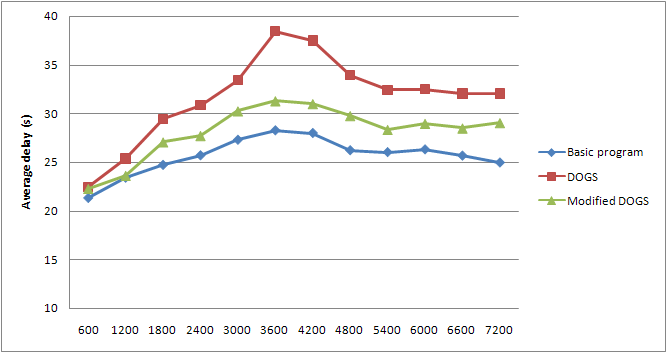
\includegraphics[scale=0.25]{delay_minor-road_glostrup.PNG}
\caption{Average delay for minor-road traffic in Glostrup}
\label{fig:delay_minor-road_glostrup}

    \end{minipage}

\end{figure}

In Vissim delays is the difference from the ideal travel time ie. no other vehicles (free flow speeds), no intersections to the actual travel time. 

We expect that delays are correlated with the queue lengths observed previously. As such we are not surprised to see that modified DOGS is the best option in Herlev for favoring arterial traffic. Original DOGS does seem to avoid the spike in average delays, which is seen in Herlev under the basic program around 8.00 (simulation second 3600) but otherwise is outperformed even by the basic program. 
For minor road traffic the differences between each program are not profound, although it is clear, as expected, that the basic program is the best choice.

In Glostrup we see that both DOGS variants reduce delays for arterial traffic and that original DOGS, on average, outperforms the modified version. For minor road traffic we see the same tendency as in Herlev, again the basic program favors this type of traffic the most whereas DOGS is hard on minor road traffic.

\subsection*{Improvements to DOGS}
These analyses leave an impression of DOGS as a system which work as intended, at best and is detrimental minor road traffic and - in some cases - even to arterial traffic as well.

The fact that minor road traffic suffers reduced performance is explained by the uneven distribution of the extra green-time, which comes as a result of increased cycle times, in the ratio 4:1. What this means is that, when DOGS increase the cycle time by 10 seconds, the arterial phase will receive 8 extra seconds of green per cycle but the minor road phase only receives 2 seconds. 
The case of performance for arterial traffic is somewhat unexpected since DOGS increased capacity and requires more study.

In the DRD report \ref{dogs} Steen Lauritzen makes a note of the uncontrolled behaviour of offsets when DOGS change level (section 5.8) and in section \ref{dogs_offset} I explained the problem.

During simulation it has been observed how the resulting poor coordinations are affected by DOGS; more vehicles are stopped at the red light due to the increased capacity and queues become longer. 

To test the theory that poor offsets are, in fact, the main cause of less-than-expected performance benefits - and even performance decreases for arterial average delays and -queues we tested a modified version of DOGS with per-cycle-time offsets. The comparisons made in the section has shown us that improper offsets are a likely cause of the performance difference and that DOGS can be improved by adopting such per-level offset values. The offset values can be calculated by any offline optimization tool, such as the one I have developed, and I believe the changes can easily be implemented in existing DOGS logic considering the easy by which I was able to change between original and modified DOGS in my VAP codes.

\subsection{Cycle times}
In Figures \ref{fig:c_dogs_herlev}-\ref{fig:c_modified-dogs_glostrup} are the cycle times chosen between 7 and 9 in the simulation.

\begin{figure}[ht]

    \begin{minipage}[b]{0.5\linewidth}

\centering
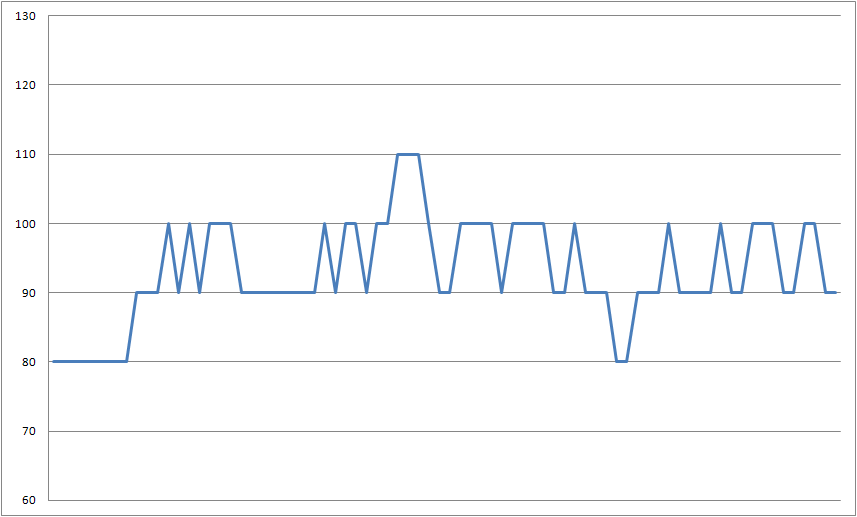
\includegraphics[scale=0.2]{C_dogs_herlev.png}
\caption{DOGS cycle time in Herlev}
\label{fig:c_dogs_herlev}

    \end{minipage}
    \hspace{0.1cm}
    \begin{minipage}[b]{0.5\linewidth}

\centering
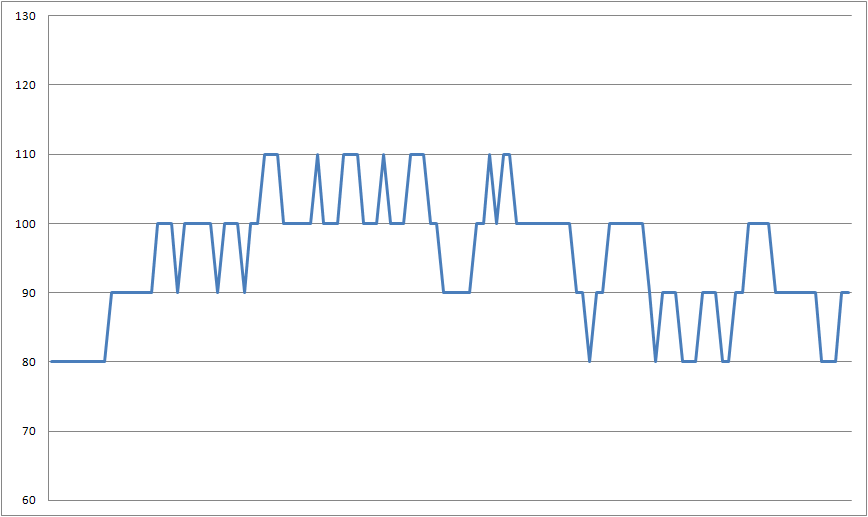
\includegraphics[scale=0.2]{C_dogs_glostrup.png}
\caption{DOGS cycle time in Glostrup}
\label{fig:c_dogs_glostrup}

    \end{minipage}
    
        \begin{minipage}[b]{0.5\linewidth}

\centering
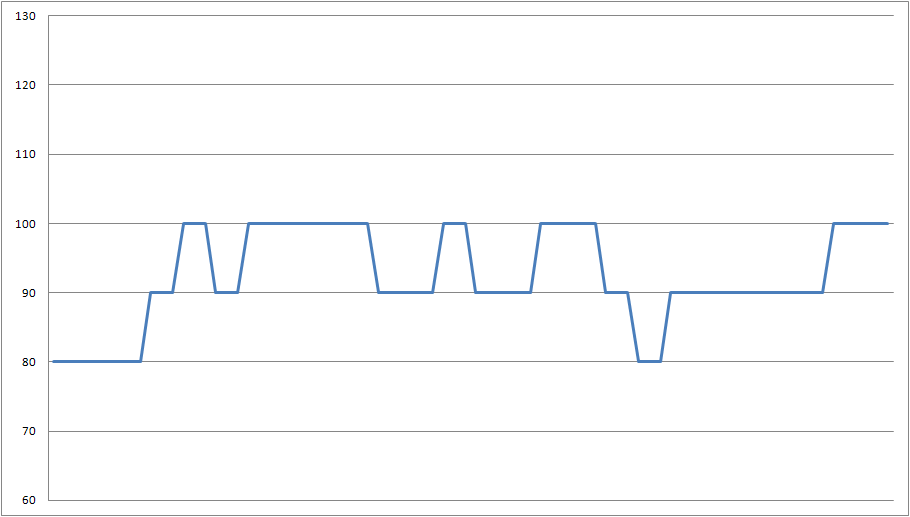
\includegraphics[scale=0.2]{C_modified-dogs_herlev.png}
\caption{Modified DOGS cycle time in Herlev}
\label{fig:c_modified-dogs_herlev}

    \end{minipage}
    \hspace{0.1cm}
    \begin{minipage}[b]{0.5\linewidth}

\centering
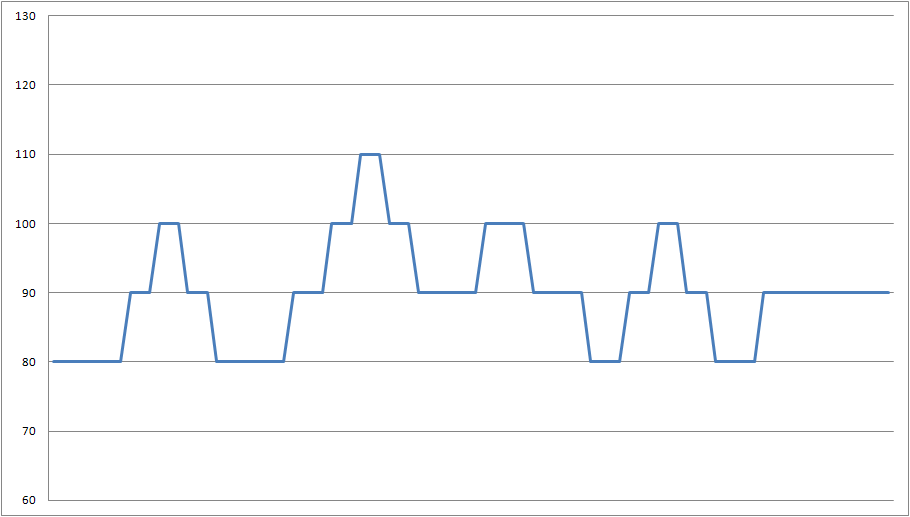
\includegraphics[scale=0.2]{C_modified-dogs_glostrup.png}
\caption{Modified DOGS cycle time in Glostrup}
\label{fig:c_modified-dogs_glostrup}

    \end{minipage}

\end{figure}

We see that the modifications made to DOGS reduces the eagerness to change levels. This is an effect of the mandatory rule for modified DOGS to remain at least 3 cycles in each level, whereas DOGS is free to change the cycle time up or down after each level has been implemented. 

This explains why modified DOGS is generally kinder on the minor roads than DOGS. Modified DOGS will remain longer at each level, allowing not only the new offsets to take effect but also the increased traffic, which caused the level change, to traverse the artery, before changing to the next level. An attempt to implement this form of level smoothening was thought into the DOGS system by the lower- and upper threshold values. However it appears that more drastic means should be taken to ensure that this of hysteria does not occur - an obvious approach is simply to require level burn-in times, such at the one I chose for modified DOGS (3 levels).

\subsection{Throughput}
DOGS attempts to increase throughput ie. the number of vehicles which traverse a section of road in the same time. The observed effect of a throughput increase is a smoothening af traffic peaks when more vehicles are let through due to increase cycle times. As we saw earlier, for instance in Figure \ref{fig:delay_arterial_herlev}, the DOGS system is capable of smoothening the average delays durings peaks of traffic (in the figure, around simulation second 3600 ie at 8-o'clock).

I have performed throughput measurements using Vissim link evaluations to see that the \textit{capacity} increase, which DOGS brings by theoretical fact, also makes an impression on the vehicle through.

The final figures \ref{fig:volume_hb-hh} and \ref{fig:volume_hh-hb} show the throughput of DOGS and modified DOGS for the road segments connecting Herlev Hovedgade and Herlev Bygade. This area was chosen since Herlev Hovedgade is considered the major bottle-neck of the Herlev area of the artery.

\begin{figure}[ht]
\centering
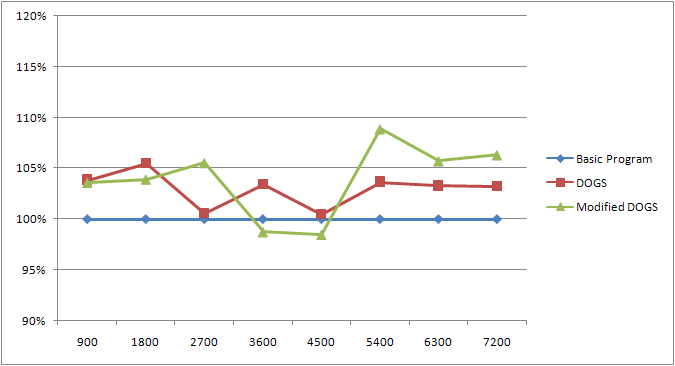
\includegraphics[scale=0.30]{volume_hb-hh.png}
\caption{Throughput over time from Herlev Bygade to Herlev Hovedgade}
\label{fig:volume_hb-hh} 
\end{figure}

\begin{figure}[ht]
\centering
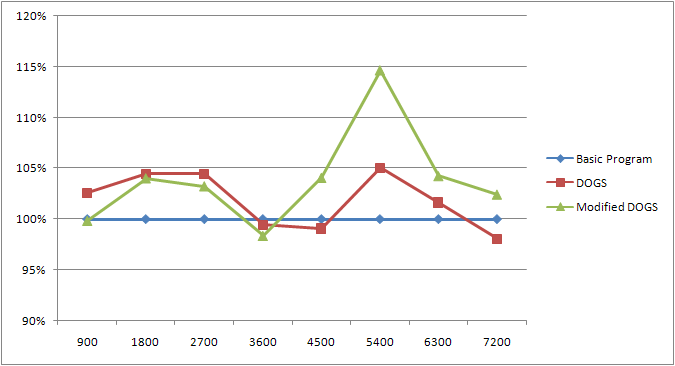
\includegraphics[scale=0.30]{volume_hh-hb.png}
\caption{Throughput over time from Herlev Hovedgade to Herlev Bygade}
\label{fig:volume_hh-hb} 
\end{figure}

Comparing the throughput of both DOGS versions to the we see that DOGS is capable of increasing the through, as expected. It appears that there is no immediate correlation between the other measurements performed on queue lengths and delays.

\subsection{Bus Priority}
The final analysis is for the bus priority for the three Glostrup intersections, Fabriksparken, Gammel Landevej and Kindebjergvej.

Bus priority is a questionable feature for a crowded arterial, such as ringroad 3. Unless there exist dedicated bus lanes, buses wait in queue to cross an intersection along with all other vehicles. For the three intersections with bus priority there is no such dedicated lane.

In Vissim it is possible to see delays per vehicle type, which in this analysis is used to filter out delays for buses.
In Figures \ref{fig:delay_bus_basic}-\ref{fig:delay_bus_modified_dogs} we see how the various systems affects bus delays with and without bus priority.

\begin{figure}[ht]
\centering
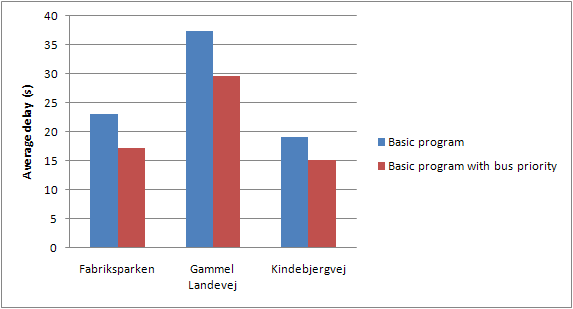
\includegraphics[scale=0.30]{delay_bus_basic.png}
\caption{Delay for buses under basic program}
\label{fig:delay_bus_basic}
\end{figure}

\begin{figure}[ht]
\centering
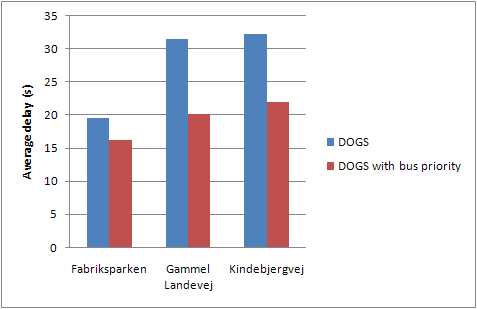
\includegraphics[scale=0.30]{delay_bus_dogs.png}
\caption{Delay for buses under DOGS}
\label{fig:delay_bus_dogs}
\end{figure}

\begin{figure}[ht]
\centering
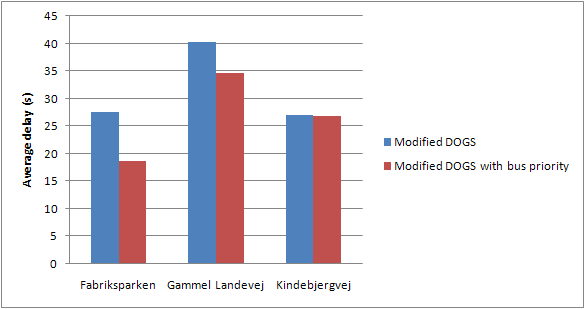
\includegraphics[scale=0.30]{delay_bus_modified-dogs.png}
\caption{Delay for buses under modified DOGS}
\label{fig:delay_bus_modified_dogs}
\end{figure}

It is clear that the bus priority logic makes a considerable positive difference in bus delay reduction. This in spite of the fact that the logic could be more aggressive by detecting waiting buses shortening the non-bus stages so that the stage, which will serve the bus, can start earlier.
